\section{Цель работы}
\begin{enumerate}
    \item Проверка основного закона динамики вращения.
    \item Проверка зависимости момента инерции от положения масс относительно оси вращения.
\end{enumerate}

\section{Задачи}
\begin{enumerate}
    \item Измерение времени падения груза при разной массе груза и разном положении утяжелителей на крестовине.
    \item Расчёт ускорения груза, углового ускорения крестовины и момента силы натяжения нити.
    \item Расчёт момента инерции крестовины с утяжелителями и момента силы трения.
    \item Исследование зависимости момента силы натяжения нити от углового ускорения. Проверка основного закона динамики вращения.
    \item Исследование зависимости момента инерции от положения масс
    относительно оси вращения. Проверка теоремы Штейнера.
\end{enumerate}

\section{Объект исследования}
Объект исследования - ускорение вращательного движения.

\section{Метод экспериментального исследования}
Многократное прямое измерение времени прохождения каретки заданного расстояния
в зависимости от массы каретки и положении утяжелителей.

\section{Рабочие формулы и исходные данные}
\begin{enumerate}
    \item Ускорение опускающегося груза $ a = \frac{2h}{t^2} $,
        где $h$ -  расстояние, пройденное грузом за время $t$ от начала движения
    \item Угловое ускорение крестовины $\varepsilon = \frac{2a}{d} $,
        где $d$ - диаметр ступицы
    \item Момент силы натяжения нити $M = \frac{md}{2} (g - a)$
    \item Расстояние между осью $O$ вращения и центром $C$ утяжелителя
        $ R = l_1 + (n-1) l_0 + \frac{1}{2}b $
    \item Стандартное отклонение $\sigma_t = \sqrt{\frac{\sum_{i=1}^n (t_i - \langle t \rangle)^2}{n}}$
    \item Погрешность измерений $\Delta t = \frac{\alpha_{0.95, n} \cdot \sigma_t}{\sqrt{n}}$
    \item Погрешность ускорения
        \[
            \Delta a =
            \sqrt{\left(\frac{\partial a}{\partial t}\right)^2 (\Delta t)^2 + \left(\frac{\partial a}{\partial h}\right)^2 (\Delta h)^2 } =
            \sqrt{\left(-\frac{4h}{t^3} \Delta t \right)^2 + \left(\frac{2}{t^2} \Delta h\right)^2}
        \]
    \item Погрешность углового ускорения $\varepsilon$:
        \[
            \Delta \varepsilon =
            \sqrt{\left(\frac{\partial \varepsilon}{\partial a} \Delta a\right)^2 + \left(\frac{\partial \varepsilon}{\partial d} \Delta d\right)^2} =
            \sqrt{\left(\frac{2}{d} \Delta a \right)^2 + \left( \frac{2a}{d^2} \Delta d \right)^2}
        \]
    \item Погрешность момента силы $M$: 
        \[
            \Delta M =
            \sqrt{\left(\frac{\partial M}{\partial m} \Delta m\right)^2 + \left(\frac{\partial M}{\partial d} \Delta d\right)^2 + \left(\frac{\partial M}{\partial a} \Delta a\right)^2} = \\
        \]
        \[
            \sqrt{\left(\frac{1}{2}d(g-a)\right) \Delta m)^2 + \left(\frac{1}{2}m(g-a) \Delta d \right)^2 + \left(- \frac{dm}{2} \Delta a\right)^2}
        \]
\end{enumerate}

\section{Измерительные приборы}
\begin{table}[ht]
    \centering
    \begin{tabular}{| c | c | c | c | c |}
        \hline
        \textnumero п/п & Наименование & Тип прибора & Используемый диапазон & Погрешность \\
        \hline
        1 & Секундомер & Цифровой & 0-20 с & 0.5 с \\
        \hline

    \end{tabular}
    \caption{Измерительные приборы}
\end{table}

\section{Схема установки}
\begin{figure}[ht]
    \centering
    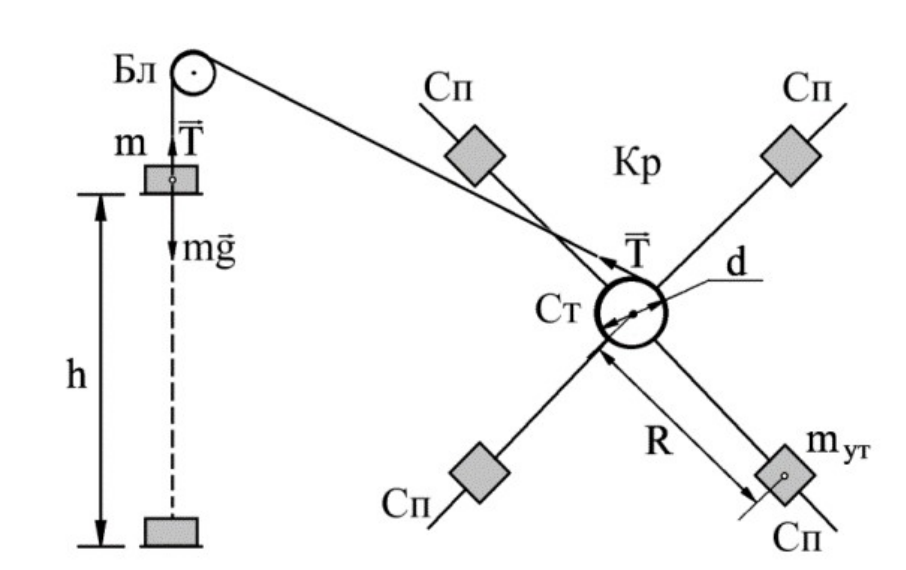
\includegraphics[width=\textwidth]{img/scheme.png}
    \caption{Схема установки}
\end{figure}
